\documentclass[11pt,a4paper]{report} 

% Für doppelseitigen Ausdruck (nur bei > 60 Seiten sinnvoll)
% \usepackage{ifthen}
% \setboolean{@twoside}{true}
% \setboolean{@openright}{true} 
%Wahrscheinlich eher nicht

% Deutsch
\usepackage[german]{babel} % deutsch und deutsche Rechtschreibung
\usepackage[utf8]{inputenc} % Unicode Text 
\usepackage[T1]{fontenc} % Umlaute und deutsches Trennen
\usepackage{textcomp} % Euro
\usepackage[hyphens]{url}
% statt immer Ab\-schluss\-ar\-beit zu schreiben
% einfach hier sammeln mit -. 
\hyphenation{Ab-schluss-ar-beit}
% Vorsicht bei Umlauten und Bindestrichen
\hyphenation{Ver-st\"ar-ker-aus-gang}
 % eigene Hyphenations, die für das Dokument gelten
\usepackage{amssymb} % Symbole
\usepackage{emptypage} % Wirklich leer bei leeren Seiten

%% Fonts, je ein kompletter Satz an Optionen

% Times New Roman, gewohnter Font, ok tt und serifenlos
%\usepackage{mathptmx} 
%\usepackage[scaled=.95]{helvet}
%\usepackage{courier}

% Palatino mit guten Fonts für tt und serifenlos
\usepackage{mathpazo} % Palatino, mal was anderes
\usepackage[scaled=.95]{helvet}
\usepackage{courier}

% New Century Schoolbook sieht auch nett aus (macht auch tt und serifenlos)
%\usepackage{newcent}

% Oder default serifenlos mit Helvetica 
% ich kann es nicht mehr sehen ...
%\renewcommand{\familydefault}{\sfdefault}

% ein bisschen eine bessere Verteilung der Buchstaben...
\usepackage{microtype}

% Bilder und Listings
\usepackage{graphicx} % wir wollen Bilder einfügen
\usepackage{subfig} % Teilbilder
\usepackage{wrapfig} % vielleicht doch besser vermeiden
\usepackage{listings} % schöne Quellcode-Listings
% ein paar Einstellungen für akzeptable Listings
\lstset{basicstyle=\ttfamily, columns=[l]flexible, mathescape=true, showstringspaces=false, numbers=left, numberstyle=\tiny}
\lstset{language=python} % und nur schöne Programmiersprachen ;-)
% und eine eigene Umgebung für Listings
\usepackage{float}
\newfloat{listing}{htbp}{scl}[chapter]
\floatname{listing}{Listing}

% Seitenlayout
\usepackage[paper=a4paper,width=14.2cm,left=36mm,height=22cm]{geometry}
\usepackage{setspace}
\linespread{1.15}
\setlength{\parskip}{0.5em}
\setlength{\parindent}{0em} % im Deutschen Einrückung nicht üblich, leider

% Seitenmarkierungen 
\newcommand{\phv}{\fontfamily{phv}\fontseries{m}\fontsize{9}{11}\selectfont}
\usepackage{fancyhdr} % Schickere Header und Footer
\pagestyle{fancy}
\renewcommand{\chaptermark}[1]{\markboth{#1}{}}
%\fancyhead[L]{\phv \leftmark}
\fancyhead[RE,LO]{\phv \nouppercase{\leftmark}}
\fancyhead[LE,RO]{\phv \thepage}
% Unten besser auf alles Verzichten
%\fancyfoot[L]{\textsf{\small \kurztitel}}
\fancyfoot[C]{\ } % keine Seitenzahl unten
%\fancyfoot[R]{\textsf{\small Technische Informatik}}

% Theorem-Umgebungen
\newtheorem{definition}{Definition}[chapter]
\newtheorem{satz}{Satz}[chapter]
\newtheorem{lemma}[satz]{Lemma} % gleicher Zähler wie Satz
\newtheorem{theorem}{Theorem}[chapter]
\newenvironment{beweis}[1][Beweis]{\begin{trivlist}
\item[\hskip \labelsep {\textit{#1 }}]}{\end{trivlist}}
\newcommand{\qed}{\hfill \ensuremath{\square}}

% Quellen teilen
\usepackage{bibtopic} 

% Hochschule Logo, noch nicht perfekt
\usepackage{hsmalogo}

% Spezialpakete
\usepackage{epigraph}
\setlength{\epigraphrule}{0pt} % kein Trennstrich

% damit wir nicht so viel tippen müssen, nur für Demo 
\usepackage{blindtext} 

% Zum Zeigen von Fehlern
\usepackage{soul}
\newcommand*\falsch{\st}

\graphicspath{{./images/}}


\usepackage{longtable}
 % alle Pakete und Einstellungen

% Hier anpassen 
\newcommand{\welchethesis}{Bachelor}
\newcommand{\thesisofwas}{of Science}
\newcommand{\studiengang}{Technische Informatik}
\newcommand{\titel}{Arbeitstitel: Anforderungen und Testen}
\newcommand{\kurztitel}{Arbeitstitel: Anforderungen und Testen}
\newcommand{\autor}{Florian Brunotte}
\newcommand{\datum}{30.01.2021} % Abgabedatum
\newcommand{\ort}{Mannheim}
\newcommand{\referent}{Prof.\ Dr.\ Ing. Mark Hastenteufel}
\newcommand{\korreferent}{Prof.\ Dr.\ Martin Damm}

\begin{document}

\begin{titlepage}
  % Kopf der Seite
  \hsmalogo[1] \hfill
  \parbox[b]{60mm}{
    % \textsf würde das Aussehen der ersten Seite ruinieren, 
    % wer will, soll das selbst außen rum machen...
    Fakultät Informationstechnik\\
    Studiengang \studiengang}
  \begin{center}
    % rumfiddeln, damit es für 4 Zeilen gerade noch so geht...
    \rule{1\textwidth}{1pt}\\[-3mm]
    \parbox[t][64mm]{110mm}{% 11 cm für Breite 13, ca. 7 für Höhe 6
      \begin{center}
        \Large{\welchethesis arbeit}\\[2mm]
        {\begin{spacing}{1.13} \huge \bfseries \titel \end{spacing}}
        \vfill
        \Large{\autor} \\[1mm] % keep space to window
        \ 
      \end{center}
    }
    \rule{\textwidth}{1pt}    
    \vfill    
    {\Large Abschlussarbeit} \\[5mm]
    {\large zur Erlangung des akademischen Grades} \\[5mm]
    {\large \welchethesis\ \thesisofwas} \\[5mm]
    \vfill    
    \begin{tabular}{ll} % Mitte der Seite
      Vorgelegt von & \autor \\
      am & \datum \\
      Referent & \referent \\
      Korreferent & \korreferent
    \end{tabular}    
    \vfill
  \end{center}
\end{titlepage}
\cleardoublepage


% Erklärung gemäß der Prüfungsordnung
\thispagestyle{empty}
\subsection*{Schriftliche Versicherung laut Studien- und Prüfungsordnung}

Hiermit erkläre ich, dass ich die vorliegende Arbeit selbstständig verfasst
und keine anderen als die angegebenen Quellen und Hilfsmittel benutzt habe.

\vspace{6em}
\noindent\begin{tabular}{p{0.37\textwidth}p{0.56\textwidth}}
\ort, \datum  & \rule{0.56\textwidth}{0.5pt}\\
              & \makebox[1cm]{\ } \autor
\end{tabular}

\vfill

\cleardoublepage

 % Titelseite, Erklärungen, etc.

\begin{abstract} 
Ziel dieser Bachelorarbeit war die Erstellung einer leichtgewichtigen Software mit der Requirements und Testcases aufgenommen werden können und durch Testruns validiert werden. (Unterschied Validierung und Verifikation?) Eingesetzt wird diese Software im Rahmen von kleinen Semesterprojekten an der Hochschule Mannheim. Geschrieben wurde sie in als Webapplikation in Python und Django während die Visualiisierung und das User Interface durch HTML und CSS erstellt wurde.
\end{abstract}

\tableofcontents %Inhaltsverzeichnis wird erstellt
\chapter{Motivation - Warum wurde diese Software geschrieben?} \label{chap:motivation}
Es ist vorzuziehen, dass...

Motivation:
Die Zielgruppe für diese Arbeit und für diese Software sind die Hochschulangehörigen, die innerhalb des Studiums Anforderungen und Tests verwalten müssen. 

Es soll eine leichtgewichtiges Softwaretool entwickelt werden zum Anforderungs- und Testmanagement. Dabei sollte man sich auf die Kernfunktionalitäten beschränken, damit man sich auf das Wesentliche konzentrieren kann, dem Schreiben von Anforderungen und dem Ausführen von Tests. Andere Softwaretools, die am Markt verfügbar sind, sind für den Einsatz in der Lehre nicht geeignet, da sie zu komplex sind und auch Geld kosten können. Sollte man nicht bezahlen, werden bestimmte Funktionen gesperrt. Insgesamt sind sie zu schwergewichtig und man verliert das eben beschriebene wesentliche aus dem Blick. Eine intuitive und simple Software, wie ,,Anforderungen und Testen (WIP)'' soll hierbei Abhilfe schaffen.

Hier werden dann noch manche Tools aufgezählt. Vielleicht mit Bilder die Limitierung und die Überfülle zeigen.

\chapter{Anforderungsanalyse - Welche Anforderungen hat das Projekt?} \label{chap:Anforderungen}

Zuerst hat Herr Hastenteufel ein Dokument mit Anforderungen gesendet. Nach Absprache per Mail wurden noch folgende Sachen geklärt:
\begin{itemize}
\item Die Kategorie für die Requirements werden erstmal als einfache Kategorien wie 1, 2, 3 realisiert. Später vielleicht Auswahl aus der Art der Requirement: Stakeholderanforderung, aber dazu nochmal in SOE reingucken

\item Die Namen Requirement, Testcase und Testrun werden benutzt, um alles einheitlich zu lassen

\item Da der Admin und der Professor als Nutzer sehr ähnlich sind, wurden die beiden Rollen mit ihren Anforderungen zusammengelegt als Professor 
\end{itemize}


Ein Klassendiagramm und ein Zustandsdiagramm wurden erstmal nicht gemacht, da sie nicht für sinnvoll gehalten wurden. Aber das wurde nochmal nachgefragt.

Es wurden ein Use Case Diagramm skizziert, mehrere Activity Diagramme, die die Use Cases verfeinern skizziert und die UIs wurden auch skizziert. Daneben wurde auch das ER-Modell schon in Draw.io gezeichnet und die Tabellen daraus wurden transformiert. Somit hat man für den Prototyp bereits ein Datenmodell mit dem man testen kann. Die Diagramme werden sich wahrscheinlich noch ändern im Verlauf des Projekts, aber für den Anfang sind sie in den Abbildungen 1, 2, 3... zu sehen. Das war der Start des Projekts.

Es wurden ebenfalls erste Skizzen zu den UIs vollzogen und abgesprochen mit dem Kunden, also Herrn Hastenteufel.
Die Rückmeldungen waren:




\chapter{Implementierung - Wie erstellt man eine Django-Applikation?} \label{chap:einf}
%So geht ein Zitat oben rechts
%das sollte auch hier stehen bleiben sonst sieht es nicht gut aus und der Text überlappt
\epigraphhead[70]{\epigraph{Documentation is like sex: 
when it is good, it is very, very good; and when it is bad, 
it is better than nothing.}{\textit{Dick Brandon}}}


%Quellen sind hier das Django und das Mozilla Tutorial
Mit PyCharm ein neues Projekt starten. Dabei wird ein neues virtual Enviroment gebildet in dem man alles installieren kann, das hat aber keine Auswirkungen auf andere Installationen, wie die Hauptinstallation von Python. Neuer Ordner wurde gebildet in dem Bachelorarbeit Ordner für den Prototyp. Als nächstes sollte man Django installieren. Im Terminal von PyCharm kann alles gemacht werden, wie Django installieren. Mit Pip install django kann man dann django installieren

Dann einfach das Tutorial machen von Django Documentation.

Django entstand in einem Nachrichtenumfeld

Man startet ein neues Django Project mit django-admin startproject name, dabei sollte der Name nicht wie django oder test heißen, das könnte zu Problemen führen
cd ./anforderungenundtesten um in den richtigen Ordner zu kommen, der die manage.py Datei enthält

über python manage.py runserver kann der Developerserver aufgerufen werden und man sieht, dass die Installation geklappt hat. Man kann hierbei auch die IP Adresse so ändern, dass alle Geräte im gleichen Netzwerk Zugriff haben.

Man erhält verschiedene Dateien beim Start eines Projects, die Funktionen der einzelnen Dateien sind in der Tabelle 111 dargestellt. 
%Tabelle mit den dateien und den Funktionen


Es gibt dabei einen Unterschied zwischen einem Projekt und einer App in Django, so kann ein Projekt mehrere Apps enthalten und eine App kann in verschiedenen Projekten enthalten sein. Man sollte auf die Wiederverwendbarkeit achten.

Hierbei kam der Begriff Boiler Code auf, der Codeabschnitte beschreibt, die wenige Änderungen haben und an vielen Stellen auftauchen können. Beispiele sind in den Listings 1 und 2 dargestellt. Man sieht in dem 1. Lisitng ein Shebang für die Programmiersprache Python, damit wird dem Compiler klar das es sich hier um Python Code handelt. Im 2. Lisiting sieht man die Basis von einem HTML Dokument. Mit diesem Template können viele verschiedene Websites generiert werden, aber diese Tags sind notwendig. %Quelle Wikipedia --> Verbesserungswürdig

Die App muss unter den installierten Apps angemeldet werden


Danach sollten die URLs definiert werden und zusammengeführt werden. Es gibt eine url Datei für das Projekt und eine für die App. Von dem Projekt kann man auch die Grundseite umleiten lassen auf die Seite der App. Die verschiedenen Routen der Seiten sind in der Abbildung 1 dargestellt. 

Es müssen auch die Befehle makemigrations und migrate angewandt werden, da sie sämtliche Änderungen an den Datenbanken und den Modellen ausführen. 

Zuletzt wird mit runserver der Development Server erstellt und zum Laufen gebracht unter der Adresse 00000 kann man dann lokal die App testen oder man kann auch für alle Geräte im gleichen Netz die App verfügbar machen. Das ist nützlich, um die Webseiten auf mobilen Geräten oder generell Geräten mit verschiedenen Displaygrößen zu testen.

Die Datenbank, in diesem Fall Postgres muss auch eingerichtet werden, dazu gibt es in settings.py die Einstellungen zu Databases. Diese müssen verändert werden, damit das Django-Projekt mit einer Postgres Datenbank funktioniert. 

Danach können die Modelle definiert werden. ORM von Python ist hierbei wichtig. Die Modelle werden aus den Tabellen, die wiederrum aus den ER-Modellen hergeleitet werden, erstellt.

Die ER-Modelle sind in der Abbildung 1 dargestellt....weiter erklären. Die Modelle sind in Abbildung 1 dargestellt... auch weiter erklären.

Nachdem man die Modelle geschrieben hat muss man das Modul noch für den Admin zur Bearbeitung freischalten bzw. registrieren. Der Admin oder Superuser muss auch erstellt werden.

Modelle in Django verfolgen die DRY Regel, also man sollte sich nicht wiederholen.

Nachdem die Modelle erstellt/geschrieben wurden, kann man mit makemigrations und migrate die Tabellen/Relationen in die Datenbank einspielen. Mit makemigrations werden die migrations erstellt als Datei um noch mal drüber zu gucken. Dabei konnte ich auch den Fehler mit dem Default DateTimeField ausbessern. Da die Migrationen nacheinander gemacht werden. Jetzt kann man bereits über den Admin die Daten einpflegen. Dazu ist zu sagen, dass das bis jetzt nur der Admin kann und die Admin Seite zwar Funktional ist, aber im Sinne von UI/Aussehen noch verbessert werden kann.




Das UI wird aber später kommen, da man erstmal einen Prototyp haben möchte der die Grundlegenden Funktionen einer  Datenbank hat: Daten eintragen, löschen, ändern und anzeigen.






\chapter{\LaTeX-Sachen} \label{chap:latex}
\section{Latex Sachen als Section}

%So geht eine Aufzählung mit Punkten
Die Ziele des Templates sind wie folgt:
\begin{itemize}
\item Beispiele der typischen Verwendung von \LaTeX\ und dessen Erweiterungen 
  geben, die viele im Rahmen von Abschlussarbeiten üblichen Anforderungen 
  abdeckt.
\item Nahe am \LaTeX-Standard halten mit wenigen weit verbreiteten 
  Erweiterungen, um problemlosen Einsatz und Erweiterbarkeit sicher zu stellen.
\item Die Einhaltung der Formalien an der Hochschule~Mannheim in der
  Fakultät Informationstechnik vereinfachen.
\end{itemize}

%so kann man Sachen durchstreichen
\falsch{durchgestrichen} angezeigt. 


%so geht referenzieren, also mit der Tilde vorne ist wiochtig sonst gibt es komische Seitenumbrüche
Nehmen Sie Kapitel 1 nicht mit dazu. Schreiben Sie Inhalte und keine
Leerphrasen. Verwenden Sie nicht das "`nächste"' oder "`folgende"' Kapitel
sondern immer als Zahl das wievielte Kapitel. 
Verlassen Sie sich auf \LaTeX\ und nummerieren Sie nie selbst sondern
referenzieren Sie. Jedes Kapitel außer das Erste muss vorkommen. 
In Kapitel~\ref{chap:latex} führen wir in die \LaTeX-Umgebung kurz ein und 
geben eine Übersicht über die Tools, die notwendig sind ein Dokument zu 
erstellen.
In Kapitel~\ref{chap:layout} stellen wir das Layout sowie einige Idiome 
zum Textsatz mit \LaTeX\ vor. 
In Kapitel~\ref{chap:bilder} besprechen wir das Einbinden und Erstellen 
von Fließobjekten wie Bilder, Tabellen und Listings.
Hinweise zum Schreibstil, mathematischem Formelsatz und zur Literatur sind 
in Kapitel~\ref{chap:stil} gesammelt.
Abschließend fassen wir in Kapitel~\ref{chap:fazit} die Vorteile und Features,
hervorzuheben sind die gute Qualität und Satz,
von \LaTeX\ für Ihre Abschlussarbeit noch einmal zusammen.


%So geht eine Tabelle
in Tabelle~\ref{tab:disteditplattform}.
\begin{table}
\centering
\begin{tabular}{|l||l|l|}
\hline
\multicolumn{1}{|c|}{\textbf{Plattform}} & 
\multicolumn{1}{|c|}{\textbf{\LaTeX-Distribution}} & 
\multicolumn{1}{|c|}{\textbf{Editor}} \\\hline\hline
Linux/Unix & TeX Live         & Texmaker, Emacs \\\hline
MacOSX     & TeX Live, MacTex & Texmaker, TeXShop \\\hline
Windows    & TeX Live, MiKTeX & Texmaker, TeXstudio \\\hline   
\end{tabular}
\caption{\LaTeX-Distributionen und Editor je Plattform}
\label{tab:disteditplattform}
\end{table}

%Damit das so anders aussieht, zum Beispiel für Befehle wie makemigrations
(zum Beispiel \verb|thesis.tex|)



%So kann man andere Schriften machen
\noindent\parbox[t]{\textwidth}{
\fontfamily{ptm}\fontsize{11}{13pt}\selectfont \ 
(Times New Roman) When Apollo Mission Astronaut Neil Armstrong first 
walked on the moon, he not only gave his famous ``one small step 
for man, one giant leap for mankind'' statement but followed it by 
several remarks, usual communication traffic between him, the other
astronauts and Mission Control. 
Just before he re-entered the lander, however, he made this 
remark \textit{Good luck Mr. Gorsky}.
}

\noindent\parbox[t]{\textwidth}{
\fontfamily{phv}\fontsize{11}{13pt}\selectfont \ 
(Helvetica) Many people at NASA thought it was a casual remark concerning 
some rival Soviet Cosmonaut. 
However, upon checking, there was no Gorsky in either the
Russian or American space programs. 
Over the years many people questioned Armstrong as to what 
the \textit{Good luck Mr. Gorsky} statement meant, but Armstrong
always just smiled.
On July 5, 1995 in Tampa Bay FL, while answering questions following 
a speech, a reporter brought up the 26 year old question to Armstrong. 
This time he finally responded. Mr. Gorsky had finally died and so 
Neil Armstrong felt he could answer the question.
}

\noindent\parbox[t]{\textwidth}{
\fontfamily{pplx}\fontsize{11}{13pt}\selectfont \ 
(Palatino) When he was a kid, he was playing baseball with a friend 
in the backyard. His friend hit a fly ball, which landed in the front 
of his neighbor's bedroom windows. 
His neighbors were Mr. \& Mrs. Gorsky.
As he leaned down to pick up the ball, young Armstrong heard 
Mrs. Gorsky shouting at Mr. Gorsky. 
\textit{Oral sex! You want oral sex?! You'll get oral sex when the 
  kid next door walks on the moon!}
}

%So gehen Fußnoten
Machen Sie Fußnoten\footnote{Das ist eine Fußnote.} immer
ohne einleitendes Leerzeichen und innerhalb des Satzes,
also nie nach einem Punkt. 
Fußnoten sind ganze Sätze mit Satzzeichen.
Fußnoten sind Inhalte, die nicht für das Verständnis 
notwendig sind\footnote{Fußnoten haben übrigens 
nichts mit Noten oder Musik zu tun.}. 
Juristen verwenden Fußnoten zur Quellenangabe. Wir
sind keine Juristen und distanzieren uns 
(nicht nur) von dieser Praxis deutlich.
Setzen Sie Fußnoten sehr sehr sparsam ein.

%so geht das Referenzieren auch auf Seiten
Referenzieren Sie innerhalb des Dokuments, zum Beispiel
auf das Kapitel~\ref{chap:bilder} in dem es unter anderem
um Bilder geht und das auf Seite~\pageref{chap:bilder}
los geht, mit \verb|\ref| (meistens) oder 
\verb|pageref| (sehr selten). 
Verwenden Sie vor dem Befehl zum Referenzieren immer
ein \verb|~|. Das ist ein nicht umbrechbares Leerzeichen
und \falsch{Kapitel \\ 1}, also der 
Zeilenumbruch vor der Nummerierung, wird vermieden.

\falsch{Es macht keinen Sinn aus irgendwelchen Gr"unden}\newline
\falsch{erscheinen sie noch so sinnvoll}\\ 
\falsch{Zeilenbr"uche im Flie"stext einzuf"uhren.}\\
\falsch{Sie}\\
\falsch{wollen eigentlich etwas anderes.}

%so kann man Sachen kursiv machen
%Abkürzungsverzeichnis vielleicht wieder nehmen
Sie sollten Abkürzungen (AKÜ) bei ersten Vorkommen definieren.
Schreiben Sie das Wort zuerst aus und dann die Abkürzung in 
Klammern. 
Danach können Sie die AKÜ verwenden. 
Meistens sollten Sie jedoch auf Abkürzungen verzichten.
Schreiben Sie lieber
\textit{beispielsweise, zum Beispiel, und so weiter, beziehungsweise}
statt \textit{bspw., z.B., usw., bzw.}.

%So gehen Bindestriche
Setzen Sie die drei verschiedenen Bindestriche -, -- und --- richtig
ein. 
Der einfache Bindestrich - wird bei Worttrennungen, 
wie AKÜ-Fimmel, eingesetzt (im Quelltext mit \verb|-|).
Der etwas längere Streckenstrich -- wird bei Streckenangaben, wie
die Strecke Mannheim--Karlsruhe oder von 10:00--11:45 eingesetzt
(im Quelltext mit \verb|--|).
Der Gedankenstrich --- ist bei Einschüben --- wie zum Beispiel
hier --- einzusetzen (im Quelltext mit \verb|---|).
\falsch{Es ist auf keinen Fall ein Leerzeichen um einen Binde - strich 
oder einen Strecken -- strich und immer ein Leerzeichen
um einen Gedanken---strich}.


%noch eine Tabelle

\begin{table}[htbp] % htbp ~ here, top, bottom, page
\centering
\begin{tabular}{|r|c|l|l|}
\hline
\textbf{Name} & \textbf{Adresse} & \textbf{Wohnort} & \textbf{Telefon} \\ 
\hline\hline
Susi Sinnlos & Eichenstrasse 5 & 12345 Unterstadt & 24927749242 \\
Horst Kurz & Schnellweg 17 & 42420 Rapid & 999 \\\hline
Jochanaan Leuchtentrager & Hochstraße zu & 666 Hell & 1-800-33845\\\hline
\end{tabular}
\caption{Adressliste}
\label{tab:meinetab}
\end{table}

Die entsprechenden vordefinierten Umgebungen heißen 
\verb|table| für Tabellen und \verb|figure| für Abbildungen. 
Mit den optionalen Argumenten \verb|htbp|, das steht für
\textit{here, top, bottom, page}, geben Sie \LaTeX\ den 
Tipp, dass Sie am liebsten das Fließobjekt \textit{hier}
an dieser Stelle haben möchten. Wenn das nicht geht, dann
eben am \textit{Anfang} der Seite, und wenn das nicht geht (weil es
zum Beispiel ein Kapitelanfang ist) ans \textit{Ende} der Seite. 
Wenn das alles nicht klappt, dann halt auf eine Extra-\textit{Seite}.
Beherzigen Sie folgende Tipps zu Fließobjekten:
\begin{itemize}
\item Jede Tabelle, jedes Bild und jedes Listing ist ein Fließobjekt.
\item Zentrieren Sie Bilder und Tabellen.
\item Jedes Fließobjekt hat eine Bildunterschrift (Caption) mit
  einem Label und wird im Text passend referenziert.
\end{itemize}
Schreiben Sie nie, \falsch{wie man unten in der Tabelle sehen kann},
da Sie nie wissen und auch nicht wissen sollen, ob die Tabelle 
wirklich \glqq weiter unten\grqq\ ist. 
Verwenden Sie statt relativer Positionsangaben Referenzen mit Zahlen,
die Sie durch das Label erhalten, wie zum Beispiel 
"`wie sie in Tabelle~\ref{tab:meinetab} sehen können"'.
Verwenden Sie kurze und prägnante Bildunterschriften, die 
nicht länger als eine Zeile lang sind. 
Alles was mehr als eine Zeile hat gehört in den Fließtext.
Sie sollten für die Fließobjekt Caption keinen Satz bilden und 
daher auch keinen Punkt am Ende haben.
Die Caption ist eine Unterschrift und gehört unter das Fließobjekt.


%So kann man Bilder in den Text bauen mit wrapfigure
\begin{wrapfigure}{r}{6cm}
  \centering
  
\includegraphics[width=4cm]{gnu}
  \caption{GNU-Logo~\cite{gnulogo,fal}}
  \label{fig:gnu}
\end{wrapfigure}
Es ist möglich, wenn auch nicht empfohlen, 
Bilder an den 
Rand einer Seite zu klatschen, wie wir das mit dem 
GNU-Logo in Abbildung~\ref{fig:gnu} gemacht haben. 
Das ganze ist ein netter Effekt für Graphiken, wie zum Beispiel ein
Logo, die nicht zum Verständnis des Texts gebraucht werden und wenig
Details aufweisen. 
Der Effekt sollte aber nicht überstrapaziert werden, 1--2 Mal 
je Abschlussarbeit sollte, wenn überhaupt, rei\-chen.
Außerdem funktioniert \verb|wrapfigure| nicht immer sehr stabil.



%So kann man Sachen fett machen
Bitte nehmen Sie \textbf{nie} JPG oder PNG für Vektorgrafiken, 
also Zeichnungen mit Linien oder anderen geometrischen Objekten,
sondern ausschließlich PDF.
Binden Sie also \textbf{nie} Vektorgraphiken verpixelt ein.


%einfach so mit pdf Endung dran machen
\begin{figure}[htb]
\centering
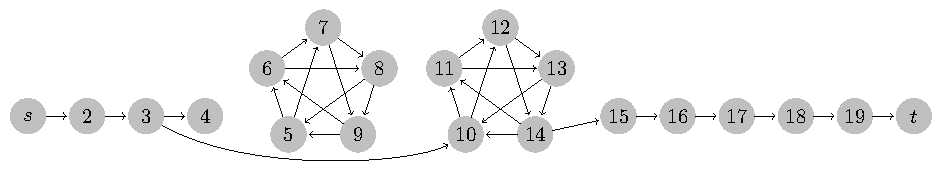
\includegraphics[width=.9\textwidth]{automata.pdf}
\caption{Automaten mit tikz~\cite{tikzautomata}}
\label{fig:tikz}
\end{figure}

%So kann man Code einbinden in 2 verschiedenen Zeichensätzen und auch aus einer Datei einlesen wie unten mit dem CPP Beispiel

Neben langen Listings sind natürlich kurze prägnante
Listings in Pseudocode (oder Python ;-) viel 
angenehmener, wie in Listing~\ref{code:ggt} der
effiziente GGT.

\begin{listing}[htbp]
\begin{lstlisting}
def ggt(x, y):
    while x != 0:
        x,y = y%x, x
    return y
\end{lstlisting}
\caption{ggT --- kurz und gut}
\label{code:ggt}
\end{listing}

Die Parameter für Listings sollte man für das ganze Dokument gleich 
lassen. 
Wenn man mal unbedingt wechseln will, dann ist das auch möglich,
wie zum Beispiel bei Listing~\ref{code:ggtjava}, das den ggT
in Java mit einem anderen Zeichensatz zeigt.

\begin{listing}[htbp]
\lstset{basicstyle=\sffamily, columns=[l]flexible, mathescape=true, showstringspaces=true, numbers=none, language=java}
\begin{lstlisting}
public static int ggt(int x, int y) {
    while (x != 0) {
        int h = x;
        x = y%x;
        y = h;
    }
    return y;
}
\end{lstlisting}
\caption{ggT --- Java}
\label{code:ggtjava}
\end{listing}

Der verwendete serifenlose Zeichensatz sieht vielleicht schöner 
aus, aber der variable Zeichenabstand kann bei Listing störend 
sein. Der in den Beispielen Listing~\ref{code:ggtaua} und 
Listing~\ref{code:ggt} verwendete Zeichensatz mit festem
Zeichenabstand ist für Quellcode meist zu bevorzugen.
Wir können natürlich auch C++-Quellcode setzen, bei Listings
\LaTeX\ in den Kommentaren verwenden und Listings aus
Dateien einlesen wie in~\ref{code:gcdcpp}.

\begin{listing}[htbp]
  \lstset{basicstyle=\ttfamily, columns=[l]flexible, mathescape=true, numbers=left, language=c++}
  \lstinputlisting{gcd.cpp}
\caption{gcd --- C/C++}
\label{code:gcdcpp}
\end{listing}


%So macht man Gänsefüßchen
Idealerweise verwenden Sie spätestens jede zweite Seite ein Bild. 
Ein Bild lockert auf und "`sagt mehr als tausend Worte"'.
Vermeiden Sie Aufzählungen.

%So macht man Mathe (falls ich das überhaupt brauche)


Eine Formel kann im Fließtext integriert sein, wie zum Beispiel 
$\sum_{i=1}^n i = \frac{n \cdot (n+1)}{2}$ oder separat
und referenzierbar gesetzt werden wie die Folgende:
\begin{equation} \label{eq:gauss}
  \sum_{i=1}^n i = \frac{n \cdot (n+1)}{2}
\end{equation}
Im \LaTeX-Quelltext werden beide Arten von Formeln gleich geschrieben 
aber anders gesetzt. 
Achten Sie zum Beispiel auf das Summenzeichen und die Positionen 
des Index. 
Die Gleichung~\ref{eq:gauss} ist natürlich vom Fließtext aus referenzierbar.
Man kann auch schreiben: 
(\ref{eq:gauss}) ist natürlich vom Fließtext aus referenzierbar.
Im Fließtext kann man auch gerne auf den Bruch verzichten und 
$\sum_{i=1}^n i = (n \cdot (n+1))/2$
schreiben, was meist etwas lesbarer ist.
Alternativ geht auch 
$\sum_{i=1}^n i = \mbox{\textonehalf} \cdot n \cdot (n+1)$.
Achten Sie bei Formeln darauf als Multiplikationszeichen 
$\cdot$ zu verwenden und nicht $*$. 
Ich kenne einen Kollegen, der ansonsten dadurch sehr erregt wird. 

Sie können viele Symbole, wie die griechischen Buchstaben 
$\alpha, \beta, \gamma, \ldots$;
logische Symbole wie $\forall, \exists, \not\exists, \wedge, \vee, \neg,
\Rightarrow, \Leftrightarrow$;
Mengensymbole wie $\in, \cup, \cap, \subseteq, \not\supset, 
\biguplus, \ldots$;
andere Symbole $\rightarrow, \sqsubseteq, \sim, 
\models, \vdash, \infty, \emptyset, \mathbb{N}, \mathbb{R}, \ldots$;
oder zusammengesetzte Gleichungen 
wie die Definition der 91er-Funktion~\cite{manna70}
verwenden.
\[
  f(x) = \left\{ \begin{array}{lll}
      x-10 & \mbox{gdw} & x>100 \\
      f(f(x+11)) & \multicolumn{2}{l}{\mbox{sonst}} 
    \end{array} \right.
\]

%So gehen dann Definitionen für Formeln

\begin{definition}
Sei $\varepsilon = 0$.
\end{definition}

\begin{satz}
Für alle positiven ganzen Zahlen $n$ gilt 
$\sum_{i=1}^n i = \frac{n \cdot (n+1)}{2}$ \enspace.
\end{satz}
\begin{beweis}
Vollständige Induktion:
\begin{itemize}
\item \emph{Induktionsanfang ($n=1$):} Es gilt  
\[
  \sum_{i=1}^1 i \, = \, 1 \, = \, \frac{1 \cdot (1+1)}{2}.
\]
\item \emph{Induktionsschritt ($n \rightarrow n+1)$:}
Es gelte die Induktionsvoraussetzung (IV):
\[
\sum_{i=1}^n i = \frac{n \cdot (n+1)}{2}
\]
Wir zeigen, dass dann auch 
\[
\sum_{i=1}^{n+1} i = \frac{(n+1) \cdot (n+2)}{2}
\]
gilt wie folgt:
\begin{eqnarray*}
  \sum_{i=1}^{n+1} i 
  & = & (\sum_{i=1}^{n} i) + (n+1)  \\
  & =_{\mbox{IV}} & \frac{n \cdot (n+1)}{2} + (n+1) \\
  & = & \frac{n \cdot (n+1)}{2} + \frac{2 \cdot (n+1)}{2} \\
  & = & \frac{n \cdot (n+1) + 2 \cdot (n+1)}{2} \\
  & = & \frac{(n+2) \cdot (n+1)}{2} 
\end{eqnarray*}
\end{itemize}
\qed
\end{beweis}
Sie müssen den Dreisatz 
\emph{Definition}, \emph{Satz} und \emph{Beweis} nicht verwenden, 
wenn Sie kein sehr formales Thema haben. 
Eine sehr formale Aufarbeitung von bekanntem Inhalt gefolgt 
von einem nicht so formalen eigenen Anteil sollte man 
meist vermeiden.

%So geht eine Website in den Text zu setzen
\url{http://www.csie.ntu.edu.tw/~cjlin/libsvm/}, 
sondern einen passenden publizierten Artikel zitieren.

%So kann man Befehle anzeigen
\begin{verbatim}
$ bibtex thesis1
$ bibtex thesis2
\end{verbatim}


\chapter{Zusammenfassung und Ausblick} \label{chap:fazit}

Abschließend kann man sagen, dass...

\newpage

% Listen wenn überhaupt ans Ende und nicht an den Anfang.
% Meist ist das aber unnötig.
% \listoffigures % Liste der Abbildungen 
% \listoftables % Liste der Tabellen
% \newpage

\bibliographystyle{plain} % Literaturverzeichnis
\begin{btSect}{thesis} % mit bibtopic Quellen trennen
\section*{Literaturverzeichnis}
\btPrintCited
\end{btSect}
\begin{btSect}{online}
\section*{Online-Quellen}
\btPrintCited
\end{btSect}
% dann mit "bibtex thesis1" und "bibtex thesis2" arbeiten

\end{document}
;;; Local Variables:
;;; ispell-local-dictionary: "de_DE-neu"
;;; End:
